Validation of the Napali approach is intrinsically linked to validation of Makai, both with synthetic benchmarks and in-situ.
Since OPQ utilizes a custom power quality measurement device, its performance needed to be characterized prior to Makai evaluation.

\section{OPQ Box Characterization.}\label{sec:opq-box-characterization.}
A mentioned in Section~\ref{subsec:software} OPQBox generates 4 metrics in order to enable event detection.
In order to evaluate the limits of detection capabilities for each one of these metrics, an OPQBox was fed with synthetic waveform generated by the SDG1025 function generator.
By utilizing a function generator the entire device including the hardware analog front end could be evaluated.
Since the function generator is not capable of supplying $120V_{rms}$ signal, a $120mV_{rms}$ signal was fed on a low side of the OPQBox resistor divider, while the device was powered via an external 5V power supply.

\subsection{Fundamental Frequency}

Fundamental Frequency computation was evaluated by generating a 60Hz sine wave via the SDG1025 and supplying it to the OPQBox.
Calculated frequency was accumulated by analyzing the device triggering stream.
The resulting histogram is shown in Figure~\ref{fig:expdes:1}
\begin{figure}[H]
    \begin{center}
        \includegraphics[width=0.6\textwidth]{img/box_eval/frequency_rms.pdf}
    \end{center}
    \caption{OPQBox frequency response.}
    \label{fig:expdes:1}
\end{figure}
As shown, the resulting distribution collected frequencies acquired over 2000s has a $\sigma=420uHz$.

\subsection{Root Mean Square Voltage}
Similarly to the fundamental frequency characterization, $V_{rms}$ calculation was evaluated by supplying the OPQBox with a 60Hz, $120mV_{rms}$ sine wave via the SDG1025.
Calculated RMS was accumulated by analyzing the device triggering stream.
The resulting histogram is shown in Figure~\ref{fig:expdes:2}

\begin{figure}[h]
    \begin{center}
        \includegraphics[width=0.6\textwidth]{img/box_eval/rms_histogram.pdf}
    \end{center}
    \caption{OPQBox $V_{rms}$ response.}
    \label{fig:expdes:2}
\end{figure}

As shown, the resulting distribution of collected $V_{rms}$ measurements, acquired over 2000s has a $\sigma=9.34mV$

\subsection{Total Harmonic Distortion}

THD performance of the OPQBox was validated by injecting a various harmonics of 60Hz superimposed onto the 60Hz, $120mV_{rms}$ sine wave into the device via the SDG1025 arbitrary waveform generation capability.
THD calculation results were acquired from the OPQBox triggering stream for analysis.
As expected resultant performance remained self-consistent across all harmonics.
Figure~\ref{fig:expdes:3} shows a histogram of the error in THD values computed from a 60Hz, $120mV_{rms}$ sinewave superimposed with a 240Hz $1.2mV_{rms}$ sine wave.
This measurement is equivalent to $1\%$ THD at the $4^{th}$ harmonic.

\begin{figure}[h]
    \begin{center}
        \includegraphics[width=0.6\textwidth]{img/box_eval/thd_rms.pdf}
    \end{center}
    \caption{OPQBox THD response.}
    \label{fig:expdes:3}
\end{figure}

As shown, the resulting distribution of collected THD measurements, acquired over 2000s has a $\sigma=0.001\%$.

\subsection{Transient Detection}

Transient detection performance was evaluated by injecting a transient superimposed onto the 60Hz, $120mV_{rms}$ sine wave into the device via the SDG1025 arbitrary function generation capability.
Transient detection results were acquired by capturing and analyzing the device triggering stream.
Transients of various shapes and magnitudes were tested.

\begin{figure}[h]
    \centering
    \begin{subfigure}{.5\textwidth}
        \centering
        \includegraphics[width=0.9\linewidth]{img/box_eval/5v_transient_rms.pdf}
        \caption{}
        \label{fig:expdes:4:1}
    \end{subfigure}%
    \begin{subfigure}{.5\textwidth}
        \centering
        \includegraphics[width=0.9\linewidth]{img/box_eval/0p5v_transient_rms.pdf}
        \caption{}
        \label{fig:expdes:4:2}
    \end{subfigure}
    \caption{Transient detection metric with a 5V transient(a), and 0.5V transient(b)}
    \label{fig:expdes:4}
\end{figure}

Figure~\ref{fig:expdes:4} shows the resultant transient detection metric for two transients.
The shape of the transient is the same and is shown in Figure~\ref{fig:opq:8:3}.
Interestingly, in case of a 0.5V transient the metric results in a much tighter distribution with $\sigma =0.015V$, while in the case of
a 5V transient the distribution exhibits a lower sideband tail.
Since the transient is injected in a random position in the cycle, and the sampling rate of the DG1025 is significantly higher then sampling rate of the OPQBox(25Msps vs 12Ksps), the peak of the transient will sometimes fall in between the consecutive samples of the OPQBox.
In the $0.5V$ transient case this effect is alleviated, since the transient is so small.
Regardless, the result shown in Figure~\ref{fig:expdes:4:2} is presented only as a synthetic benchmark, since OPQBox is expected to operate in an environment with THD larger then $0.4\%$ at $>400Hz$ required to detect a $0.5V$ transient.
As such, the figure of $\sigma=0.125V$ should be considered valid for the OPQBox transient detection capability.
Since this metric is only used in transient detection and not characterization, it was found to be sufficient.

\section{Napali Validation}\label{sec:napali-validation.}

Napali was validated using simulation, synthetic data with the device-in-loop, and in-situ during the deployment.


\subsection{Selection of $\alpha$ parameter}\label{subsec:selectrion-ofparameter}

The main tunable parameter in Napali is the $\alpha$ coefficient used in the low pass filter as shown in Equation \ref{eq:iir_mean}.
This parameter determines the memory of the lowpass filter used in the calculation of the mean and the standard deviation of metrics from OPQBox data stream.
These statistics are in turn used during the Napali triggering process to locate sub-threshold gridwide events.

A smaller $\alpha$ parameter corresponds to a longer memory in the low pass filter as shown in Equation \ref{eq:iir_alpha}.
This is further visualized in Figure \ref{fig:expdes:5}.
In particular this Figures \ref{fig:expdes:5:1} and \ref{fig:expdes:5:2} show the response of the IIR low pass filter to the simulated frequency measurements.
The dashed red line represents the frequency measurement, solid red line represents the filtered mean, and the blue line represents the standard diviation.
Figures \ref{fig:expdes:5:1} shows the filter response for $\alpha = 0.5$ or $T_{memory} \approx 10s $.
As evident from the plot, the mean and the standard deviation quickly recover from the transient are return to their nominal values.
Furthermore, the mean is closely tracking the random fluctuations present in the measurement.
Figures \ref{fig:expdes:5:1} shows the filter response for $\alpha = 0.05$ or $T_{memory} \approx 123s $.
While the stimuli remains the same, it takes significantly longer the statistics to recover.
Additionally, the mean no longer tracks the frequency fluctuations present in the simulated data.

\begin{figure}[h]
    \centering
    \begin{subfigure}{0.9\textwidth}
        \centering
        \includegraphics[width=1\linewidth]{img/napali_eval/Napali_response_freq_05.pdf}
        \caption{}
        \label{fig:expdes:5:1}
    \end{subfigure}%

    \begin{subfigure}{0.9\textwidth}
        \centering
        \includegraphics[width=1\linewidth]{img/napali_eval/Napali_response_freq_005.pdf}
        \caption{}
        \label{fig:expdes:5:2}
    \end{subfigure}
    \caption{$\mu$ and $\sigma$ behaviour with a)$\alpha = 0.5$ and b)$\alpha=0.05$}
    \label{fig:expdes:5}
\end{figure}

Picking the $\alpha$ parameter for Napali is extremely domain specific, as it depends on the frequency content of the triggering stream.
Intuitively, the $T_{memory}$ parameter needs to be long enough to adjust to gradual changes in the triggering stream for the mean calculation,
and dampen the standard deviation for detection of multiple consecutive anomalies.
In addition, it needs to be short enough to converge on the mean and the standard deviation during a step-like transition in the triggering stream.

Luckily, in the Power Quality domain the Napali $\alpha$ selection is fairly forgiving.
This is demonstrated in Figure \ref{fig:expdes:6}.
This graph represents the amount of time that Napali considered one of the metrics to be outside of the $3\sigma$ of the mean for various values of $\alpha$.
The triggering stream used to generate these values was captured over 24 hours by one of the OPQBoxes deployed on the University of Hawaii campus.
All devices deployed thus far have followed a similar pattern.
With $20s <T_{memory} < 2Hr$ the triggering stream resulted in similar behaviour, with the system correctly marking all potential sub-threshold events.
At $T_{memory} \approx 20s$, system quickly recovered from large jumps in the triggering stream, however it marked a significant number of small anomalies ($\Delta_{f}>0.01Hz$, $\Delta_{v}> 0.1V$\ldots etc) as outside $3\sigma$, and thus candidates for sub-threshold events.
At $T_{memory} \approx 2Hr$, system took  significant amount of time to recover from large jumps in triggering metrics, thus marking the metric as outside of $3\sigma$ for many tens of minutes.
Furthermore, some of the larger anomalous measurements ($\Delta_{f}>0.05Hz$, $\Delta_{v}> 2V$\ldots etc) were no longer flagged as sub-threshold candidates.
Outside of the two extremes, the system behaviour was quite similar.
During all of the deployments the OPQ system was operating with:
\begin{equation}\label{eq:opq_alpha}
\begin{aligned}
    \alpha = 0.05
\end{aligned}
\end{equation}


Which corresponds to the $T_{memory} \approx 2$ minutes.
Thresholds which initiate the Napali event detection state machine are shown in Table \ref{tbl:opq:thresholds}.

\begin{figure}[h]
    \centering
        \includegraphics[width=1\linewidth]{img/napali_eval/a_selection.pdf}
    \caption{Amount of time a metric spends outside of the $3\sigma$ for various values of $\alpha$}
    \label{fig:expdes:6}
\end{figure}

The effect of the of selecting alpha as shown in Equation \ref{eq:opq_alpha} can be observed in Figure \ref{fig:expdes:7}.
This figure shows interesting features from the same dataset that was used to produce Figure \ref{fig:expdes:6}.
Blue traces show metrics that exhibit anomalous behaviour, while red indicates that Napali has flagged this temporal region as a sub-threshold event candidate.
Figure \ref{fig:expdes:7:1} shows a frequency fluctuation which nearly passes the threshold of $60.1Hz$ which would mark it as a full fledged event.
Instead, Napali marked almost the entirety of the fluctuation as a potential sub-threshold event, as shown by the red trace.
Figure \ref{fig:expdes:7:2} shows a step in the total harmonic distortion metric, similar to the one shown in Figure \ref{fig:opq:7} at the 6am mark.
In this case the metric in question abruptly changed to a new mean, requiring a fairly slow $\alpha$ coefficient to catch up over 3 minutes.
While it may seem wasteful to mark large temporal regions following an abrupt jump as candidates for sub-threshold event, it is important to note that:
\begin{enumerate}
    \item Making the $\alpha$ parameter smaller does not benefit the false positive rate as shown in Figure \ref{fig:expdes:6}.
    \item In-situ there is no way to tell if an abrupt shift is a switch to a new steady state, or if the metric will recover to a previous mean.
\end{enumerate}
It is important to remember than Napali is not meant to have a low false positive rate.
Instead, a system like OPQ Mauka can use all available information, including the raw data, to determine if an event is true gridwide event with much higher confidence.
The main goal of Napali is to have an extremely low rate of false negatives.
Figure \ref{fig:expdes:7:3} is on a different timescale from Figures \ref{fig:expdes:7:2} and \ref{fig:expdes:7:1}.
This is done in order to include several potential sub-threshold events into a common chart.
Five temporal regions during the the 3 Hrs are marked by Napali as potential sub-threshold events.
\begin{figure}[h]
    \centering
    \begin{subfigure}{0.5\textwidth}
        \centering
        \includegraphics[width=1\linewidth]{img/napali_eval/napali_live_f.pdf}
        \caption{}
        \label{fig:expdes:7:1}
    \end{subfigure}%
    \begin{subfigure}{0.5\textwidth}
        \centering
        \includegraphics[width=1\linewidth]{img/napali_eval/napali_live_thd.pdf}
        \caption{}
        \label{fig:expdes:7:2}
    \end{subfigure}

    \begin{subfigure}{0.5\textwidth}
        \centering
        \includegraphics[width=1\linewidth]{img/napali_eval/napali_live_rms.pdf}
        \caption{}
        \label{fig:expdes:7:3}
    \end{subfigure}%
    \begin{subfigure}{0.5\textwidth}
        \centering
        \includegraphics[width=1\linewidth]{img/napali_eval/napali_live_trans.pdf}
        \caption{}
        \label{fig:expdes:7:4}
    \end{subfigure}

    \caption{Potential sub-threshold events for a) $f_{fundamental}$, b)$THD$, c)$V_{rms}$ and d)$Trans$.
    Red boxes indicate that Napali picked these temporal windows as a potential sub-threshold event.}
    \label{fig:expdes:7}
\end{figure}

\subsection{Sub-Threshold Event Detection}\label{subsec:sub-threshold-event-detection}

One of the main goals of Napali is to utilize metric extraction in order to detect sub-threshold events.
During the deployment, two types of sub-threshold events have been identified:
\begin{itemize}
    \item Partial sub-threshold event.
    \item Full sub-threshold event.
\end{itemize}
Full sub-threshold events consist of one or several devices passing the threshold described in Table \ref{tbl:opq:thresholds},
as well as one or several devices marked as sub-threshold by Napali.
Partial sub-threshold events consist of devices which all passed the threshold described in Table \ref{tbl:opq:thresholds}, however some of the devices triggered on a different metric with a much shorter temporal window.
The important distinction between partial sub-threshold events and regular events is that if triggered using the Self-Triggering method, the majority of the sub-threshold data would be lost.

\begin{figure}[h]
    \centering
    \begin{subfigure}{1\textwidth}
        \centering
        \includegraphics[width=1\linewidth]{img/napali_eval/rms_gridwide_subthreshold.pdf}
        \caption{}
        \label{fig:expdes:8:1}
    \end{subfigure}%

    \begin{subfigure}{1\textwidth}
        \centering
        \includegraphics[width=1\linewidth]{img/napali_eval/raw_gridwide_subthreshold_zoom.pdf}
        \caption{}
        \label{fig:expdes:8:2}
    \end{subfigure}
    \caption{Partial sub-threshold event a) the sub-threshold component of the event, b) above threshold component of the event}
    \label{fig:expdes:8}
\end{figure}

An example of a partial sub-threshold event is shown in Figure \ref{fig:expdes:8}.
Figure \ref{fig:expdes:8:1} shows the sub-threshold component of the event.
In this event device 2 passed the threshold on $V_{rms}$ metric, initiating Napali to look for sub-threshold events across other devices.
It is important to note, that at the event start device 1 was considered to be a sub-threshold candidate, however, at $t \approx 26.8s$ device 1 produced a transient metric which was above napali threshold.
As such Napali requested raw data from both device 1 and device 2, creating a partial sub-threshold event containing both a voltage sag shown in Figure \ref{fig:expdes:8:1} and a transient shown in Figure \ref{fig:expdes:8:2}.

\begin{figure}[h]
    \centering
    \begin{subfigure}{0.49\textwidth}
        \centering
        \includegraphics[width=1\linewidth]{img/napali_eval/raw_gridwide_sub_full1.pdf}
        \caption{}
        \label{fig:expdes:9:1}
    \end{subfigure}%
    \begin{subfigure}{0.49\textwidth}
        \centering
        \includegraphics[width=1\linewidth]{img/napali_eval/raw_gridwide_sub_full2.pdf}
        \caption{}
        \label{fig:expdes:9:2}
    \end{subfigure}

    \begin{subfigure}{0.49\textwidth}
        \centering
        \includegraphics[width=1\linewidth]{img/napali_eval/raw_gridwide_sub_full3.pdf}
        \caption{}
        \label{fig:expdes:9:3}
    \end{subfigure}
    \begin{subfigure}{0.49\textwidth}
        \centering
        \includegraphics[width=1\linewidth]{img/napali_eval/raw_gridwide_sub_full4.pdf}
        \caption{}
        \label{fig:expdes:9:4}
    \end{subfigure}
    \caption{Full sub-threshold event across 4 devices.
    a) Device 1: above threshold b) Device 2: sub-threshold c) Device 3: above threshold d) Device 4: above threshold.}
    \label{fig:expdes:9}
\end{figure}

An example of a full sub-threshold event is shown in Figure \ref{fig:expdes:9}.
This is a short-lived transient event observed by four devices on September 5\textsuperscript{th}.
Devices 1, 3, and 4 generated a transient metric higher then the Napali threshold.
Device 2 transient metric did not pass threshold, yet nonetheless produced a severe enough deviation from the mean for Napali to consider it a part of the event.
This is particularly evident in the mild transient observed in Figure \ref{fig:expdes:9:2}.

\section{University of Hawaii Deployment.}\label{sec:university-of-hawaii-deployment.}

As part of the Napali validation, the OPQ system was deployed across the University of Hawaii Manoa campus (UH).
This location was advantageous because it is an isolated microgrid connected to the Oahu powergrid only via a single 46kV feeder as shown in Figure~\ref{expdes:fig:1}.
Another advantage of the UH campus is the high number of smart meters deployed across various levels of the power delivery infrastructure.
While the purpose of these meters is monitoring the power consumption, they do include some rudimentary power quality monitoring capabilities.
Data from the campus deployed meters was used as ground truth for comparison against the measurements, and for analysis performed by the OPQ project.
The location of smart meters in the grid topology is shown in Figure~\ref{expdes:fig:1} as the $M$ nodes.
As evident by the meter location none of them were monitoring the consumer level power and mainly focused on the higher voltage power delivery.
This placement was a consequence of the smart meters role as a consumption monitor, and thus the deployment of the OPQ Boxes at the residential level complimented UH power quality monitoring capabilities without introducing redundancies.

University of Hawaii power grid is supplying a highly diverse infrastructure.
Beyond the traditional residential equipment such as computers and consumer grade electronics, the UH power grid powers scientific and laboratory equipment, machine shops, and server farms.
All of these elements have varying requirements/tolerances for power quality anomalies as well as different levels of power quality ``pollution''.
Furthermore, some of the electricity consumers in the UH campus are entirely unique.
For example, the free electron laser located in the Watanabe Hall is one of the only free electron lasers in the world, and the impact/sensitivity of power quality on the instrument are completely unstudied.
\begin{figure}[h]
    \centering
    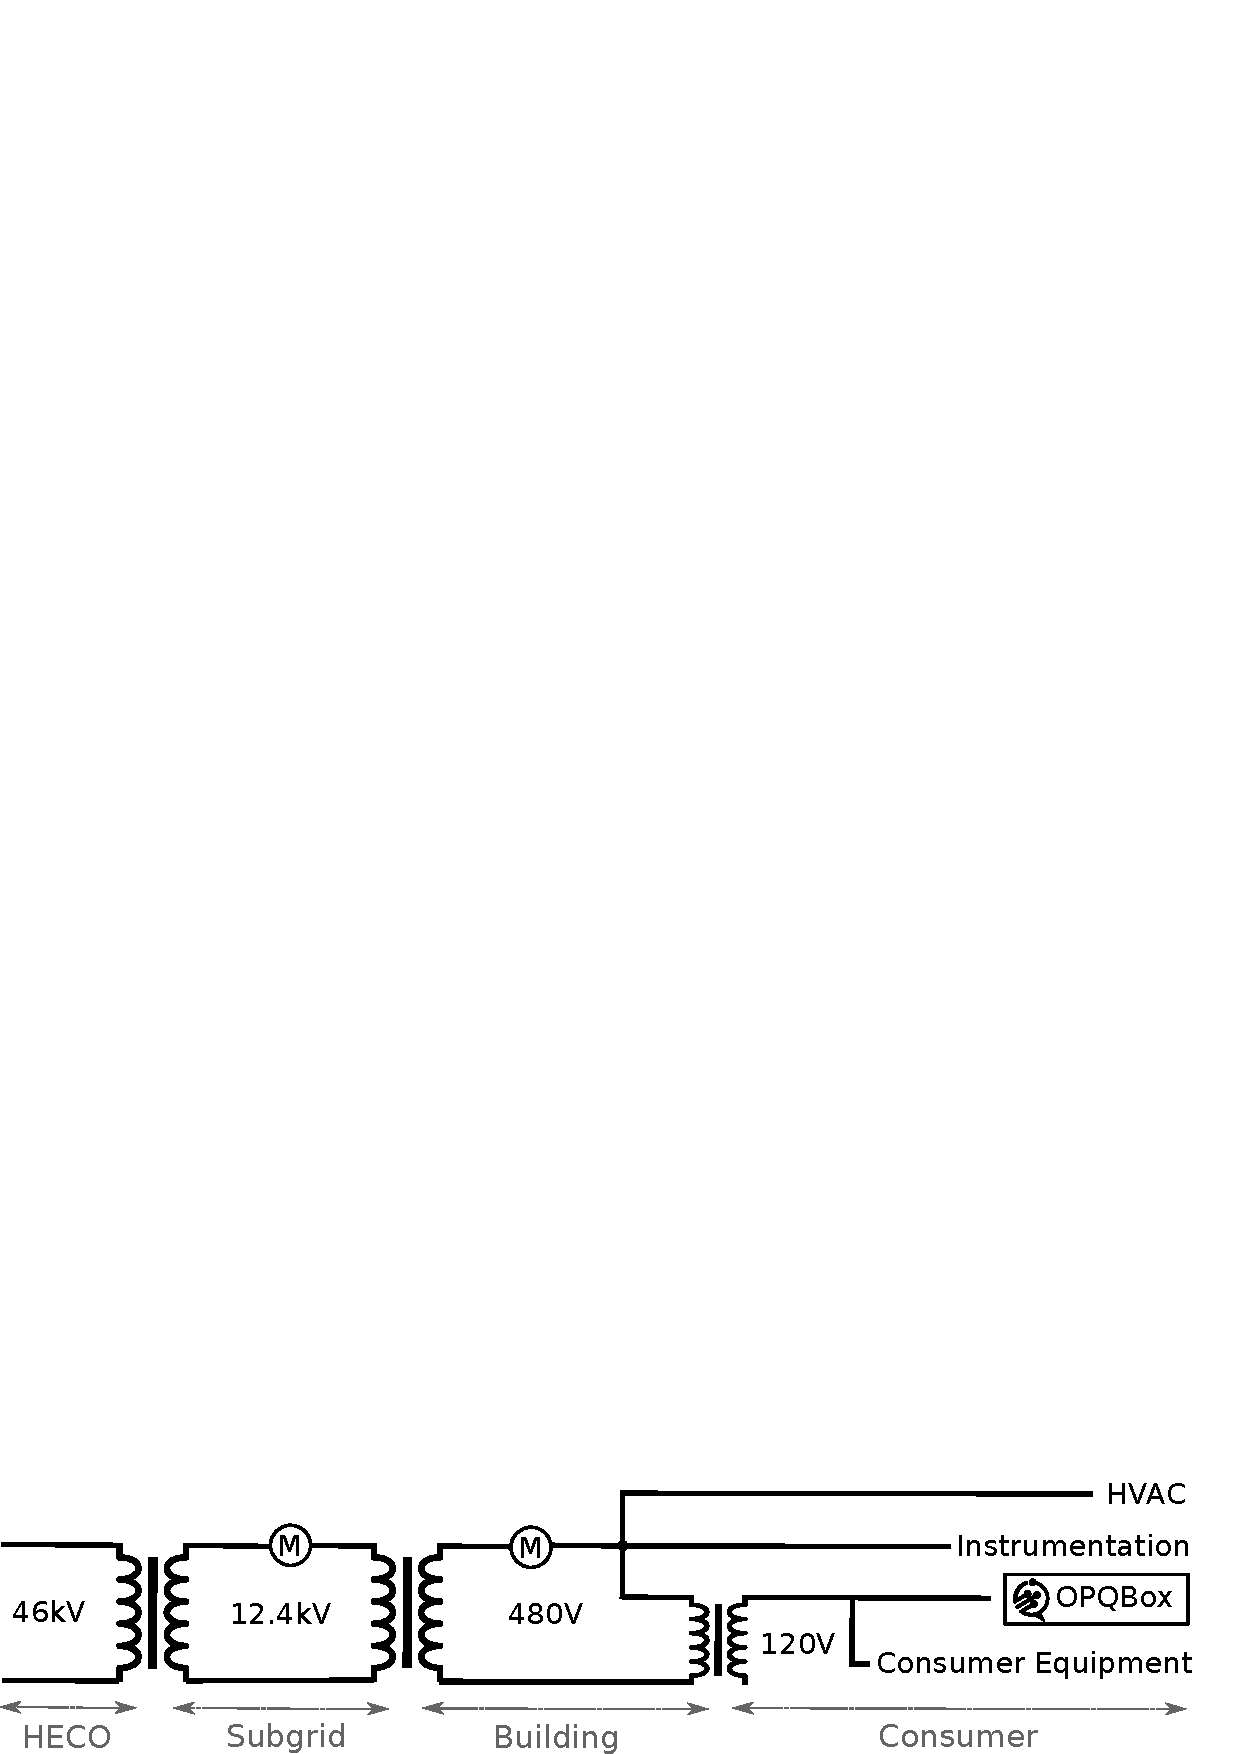
\includegraphics[width=1\linewidth]{img/uh-grid.pdf}
    \caption{University of Hawaii at Manoa power delivery infrastructure.}
    \label{expdes:fig:1}
\end{figure}

There are 74 smart meters deployed across the UH campus.
These meters measured the fundamental frequency $V_{rms}$, power consumption, reactive power, and power factor.
Data from these meters was cross-referenced with the Napali detection system in order to ascertain it's benefits.

OPQ Box placement was specifically selected to cover as much of the University of Hawaii power delivery infrastructure as possible.
The OPQ Box deployment is shown in Figure \ref{expdes:fig:deploy}.
By spreading out devices across the entire power grid, OPQ system is able to monitor the propagation of power quality disturbances throughout the UH power grid.
Consider the event shown in Figure \ref{fig:expdes:9}.
Figure \ref{expdes:fig:grid_wide_filtered} shows the same event with the fundamental and harmonics suppressed using a notch filter bank.
Furthermore, the location annotation is added to indicate the device location.
The most affected devices were located at the Physical Plant and Hamilton Library, recording a $~60V_{pp}$ transient.
Incidentally, both of these devices are monitoring a subgrid rooted at transformer(MA4).
Another device recorded this event was located in Watanabe Hall.
This device recorded a $30V_{pp}$ transient, still above the threshold for detection.
This device was monitoring the the subgrid rooted at the transformer LA4.
The final device was located at the parking structure entirely across campus.
This device recorded a $15V_{pp}$ transient, about 1V below the required magnitude for the threhold based detection.
However, Napali was able to determine that the parking structure OPQ Box was affected by the disturbance, and requested the raw data regardless.

\begin{figure}[h]
    \centering
    \includegraphics[width=1\linewidth]{img/deployment/gridwide_locality.pdf}
    \caption{Filtered Transient from event shown in Figure \ref{fig:expdes:9}}
    \label{expdes:fig:grid_wide_filtered}
\end{figure}

From the data gathered by Napali as shown in Figure \ref{expdes:fig:grid_wide_filtered}, it seems apparent that the disturbance originated at the subgrid rooted at the transformer MA4.
The Watanabe device was affected due to the short geographic and electrical distance to the MA4 subgrid.
By the time transient reached the parking structure, it was significantly attenuated by the transformers and transmission lines.
It was only detected due to the sub-threshold detection ability of the Napali framework.
\clearpage
\begin{figure}[h]
    \centering
    \includegraphics[width=0.7\linewidth]{img/deployment/uh_power_grid.pdf}
    \caption{OPQ Box locations and device IDs across University of Hawaii.}
    \label{expdes:fig:deploy}
\end{figure}

\clearpage

\subsection{Napali Bandwidth usage}\label{subsec:napali-bandwidth-usage}
During the OPQ deployment it was found that Napali significantly outperformed both the Self-Triggered and the Naive event detection methods.
In order to evaluate the bandwidth performance of Napali a Self-Triggered plugin ran along side it inside the Makai host.
This plugin utilized the same thresholds as Napali as described in Table \ref{tbl:opq:thresholds}.
However, the Self-Triggered plugin did not take into the account any inter-device signatures.
This method is equivalent to each the device performing non-collaborative triggering.
\begin{figure}[h]
    \centering
    \includegraphics[width=0.8\linewidth]{img/napali_eval/napali_request_bandwidth.pdf}
    \caption{Amount of data requested from 10 OPQ Boxes via the Self-Triggered and Napali methods.}
    \label{expdes:fig:self_triggered_bandwidth}
\end{figure}

Figure \ref{expdes:fig:self_triggered_bandwidth} shows the amount of data requested from 10 devices by the Self-Triggered and Napali plugins over 24 Hours.
It is evident, that the majority of data requests for the Self-Triggered method resulted in local noise, and did not contribute to the grid measurements.
Napali on the other hand, ignored anomalies which did not affect more then a single device, while requesting sub-threshold data during a gridwide PQ event.

\begin{figure}[h]
    \centering
    \begin{subfigure}{.5\textwidth}
        \centering
        \includegraphics[width=1\linewidth]{img/napali_eval/napali_metric_bandwidth.pdf}
        \caption{}
        \label{expdes:fig:napali_metric_bandwidth}
    \end{subfigure}%
    \begin{subfigure}{.5\textwidth}
        \centering
        \includegraphics[width=1\linewidth]{img/napali_eval/napali_cmd_bandwidth.pdf}
        \caption{}
        \label{expdes:fig:napali_cmd_bandwidth}
    \end{subfigure}
    \caption{Penalties incurred by the Napali framework.
    a) Metrics received from 10 OPQ Boxes.
    b) Commands sent to 10 OPQ Box }
    \label{expdes:fig:napali_bandwidth_penalty}
\end{figure}

It should be noted that the Self-Triggered method does not incur the penalty of having to constantly transmit the device metrics to the sink, since all the event detection is performed on the device.
Figure \ref{expdes:fig:napali_metric_bandwidth} shows the amount of data received via metrics from 10 OPQ Boxes during the same 24 hours as the Figure \ref{expdes:fig:self_triggered_bandwidth}.
As expected the bandwidth requirement for metric transmission remains constant, since all OPQ Boxes send the metrics at fixed intervals.
While this penalty is significant as it constitutes 41\% of the total bandwidth used by Napali, the aggregate bandwidth is still shows a 440\% improvement over the Self-Triggered method.
Another penalty incurred by Napali is the two way communication requirement.
Each device which participated the event detection needed to receive a command with the temporal range which anomalous data.
Neither the Naive nor Self-Triggered methods require two-way communication, and as such there is no direct comparison to Napali.
Figure \ref{expdes:fig:napali_cmd_bandwidth} shows the command bandwidth consumption for 10 OPQ Boxes across 24 hours.
The total consumption was ~50kB, which is quite trivial for any modern sensor network.

During the 24 hours of shown in Figures \ref{expdes:fig:napali_bandwidth_penalty} and \ref{expdes:fig:self_triggered_bandwidth}, Napali captured 60 events, while the Self-Triggered method captured 878.
The average length of the Napali Event was 10s to the Self-Triggered 3s.
Of 60 Napali events, all 60 contained sub-threshold data.

Comparison of Napali with the Naive method was performed analytically.
Since the sampling rate of the OPQ Box is well characterized, and the number of OPQ Boxes is fixed, it is trivial to calculate the amount of raw data generated by the OPQ network during any time period.
In order to make this comparison fair, the raw data bandwidth will be scaled by the compression ratio of the state of the art compression algorithm specifically designed for power quality measurements.\cite{zhang2009new}
Operating at 12kSps, OPQ Box produces raw data at 24KB/s.
With state of the art compression operating at 90\% compression ratio and 5\% overhead of meta-data, one can expect a ~3KB/s stream of raw data for each OPQ box if it were to send the entirety of it to the sink.
For 10 OPQ Boxes we would expect the aggregate bandwidth of 30kB/s, and as such the bandwidth consumption 24.7GB/day.
During a 24 hour period, as shown in Figures \ref{expdes:fig:napali_bandwidth_penalty} and \ref{expdes:fig:self_triggered_bandwidth}, Napali used 234MB of bandwidth.
This corresponds to an over 100x improvement over the Naive method.

\begin{figure}[h]
    \centering
    \includegraphics[width=0.8\linewidth]{img/napali_eval/napali_bandwidth_comparison.pdf}
    \caption{Bandwidth requirement comparison between three event detection methods.}
    \label{expdes:fig:bandwidth_master_comparison}
\end{figure}

Figure \ref{expdes:fig:bandwidth_master_comparison} shows the comparison between Napali as well as the Naive and Self-Triggered methods.
While Napali incurs additional costs described in Figure \ref{expdes:fig:napali_bandwidth_penalty} it outperforms the comparable methods.
Finally, the cost of the two way communication as shown in Figure \ref{expdes:fig:napali_cmd_bandwidth} is greatly outweighed by the bandwidth savings in the raw data reception.
Modern sensor networks greatly benefit from two way communication, as it allows on-demand health monitoring, and software updates.
With addition of Napali, two way communication allows for significant bandwidth requirement reduction in for the sensor network as a whole.

\subsection{Sink processing requirement under the Napali Framework}\label{subsec:sink-processing-requirement-under-the-napali-framework}
Sink processing requirements for event detection between Self-Triggered, Naive and Napali are quite different.
In general the processing requirement can be described as follows:
\begin{equation}\label{eq:detection_cost}
\begin{aligned}
    C_{total} = C_{metric\_extraction} + C_{detection}
\end{aligned}
\end{equation}

In the Equation \ref{eq:detection_cost} the $C_{total}$ is the total cost, $C_{metric\_extraction}$ is the cost of extracting metrics and $C_{detection}$ is the cost of event detection.\cite{de2015effective}
Each of the three methods, Napali, Self-Triggered, and Naive, has different sink costs associated with each parameter.

\subsubsection{Sink processing: Naive Method}

First, let's consider the Naive method.
In this case all of the metrics need to be extracted at the sink.
Disregarding the processing power required to keep up with the data rate described in Section \ref{iexp:sec:band} the $C_{feature\_extraction}$ can be measured empirically.
In order perform this measurement, OPQ Box software was built for an x86 architecture and stress-tested.
Instead of acquiring data from a device driver, the feature extraction stack was supplied with synthetic data.
Finally, the ZMQ communication was removed and replaced with the performance analysis code.
Stress test was performed on a Intel Core i9-8950HK CPU with thermal management disabled running at 2.9GHz.
Under such conditions, the metric extraction stack was able to extract features from 1s worth of raw data in $800us$ running on a single core.
Since metric extraction has no inter-device data dependencies, a modern 8 core CPU can expect to keep up with feature extraction from 1000 devices.
If an OPQ Box sensor is used with 16 bit samples and 12kSps ADC, aggregate bandwidth for such system is 10.8Gbps, which is well within the realm of a collocated server with dual 10Gbps network interfaces.
$C_{detection}$ cost can be made linear with the number of devices.
If a rolling window is applied to metrics as they are generated, raw data from all devices contained in the window with an offending threshold metric can be retained for later analysis.
While simple, this method will collect all of the gridwide events along with a large number of false positives.
In synthetic benchmarks, the $C_{detection}$ made up less then $0.01\%$ of the computational cost when compared to $C_{feature\_extraction}$
and does not significantly contribute to the $C_{total}$.

\subsubsection{Sink Processing: Naive Method}

In contrast to the Naive method, the Self-Triggered method, has no sink processing requirements, since all of the feature-extraction is performed on the edge device.
Thus, Self-Triggered method event detection is only limited by the available network bandwidth.

\subsubsection{Sink Processing: Napali Method}

Napali, being a hybrid of Naive and Self-Triggered methods, moves the $C_{metric\_extraction}$ cost to the edge devices, while retaining
the $C_{detection}$ at the sink.
Unlike the Naive case, napali performs additional computations on the features in order to detect sub-threshold events while excluding the local noise.
However, even with additional metric analysis the Napali stack was able to process synthetic data from 100000 devices on a single core of an a Intel Core i9-8950HK CPU.
This would allow a single server running Makai to provide 50\% coverage of households in the city of Honolulu.

\subsubsection{Sink Processing: Event Classification}

The final step of any power quality analysis stack is event classification.
Every event collected by an event detection system must be analyzed and classified according to their severity and type.
While Makai/Napali are not responsible for event classification it is important to consider the event classification cost when discussing sink processing requirements.
In the case of the Naive method, events which are detected are a mix of local and global events.
However, every event will contain a waveform from every device on the network.
For the Self-Triggered method, only the events which cross the threshold will be considered for classification.
While Self-Triggered events will not contain false positives and sub-threshold events, vast majority of acquired waveforms are comprised of local disturbances.
Finally, Napali produces high quality events which only contain high fidelity sub and over threshold events, while ignoring local disturbances.
During the campus deployment Napali detected 302 Events comprised of 1561 individual device waveforms a week on average.
The Self-Triggered method detected 26520 offending waveforms.
If we assume unitary classification cost, classification computational requirements for one week of data are shown in Figure \ref{expdes:fig:classification}.
\begin{figure}[h]
    \centering
    \includegraphics[width=0.8\linewidth]{img/napali_eval/classification_cost.pdf}
    \caption{Classification cost based on the expected amount of waveforms for the three considered methods.}
    \label{expdes:fig:classification}
\end{figure}


\subsection{Effects of latency in the Napali framework}\label{subsec:effects-of-latency-in-the-napali-framework}

In order to understand the effects of latency on Makai in the OPQ deployment, we examined the event length and round trip latency for OPQ Boxes.
These parameters are shown in Figure \ref{expdes:fig:el_la}.

\begin{figure}[h]
    \centering
    \begin{subfigure}{.45\textwidth}
        \centering
        \includegraphics[width=1\linewidth]{img/napali_eval/event_length.pdf}
        \caption{}
        \label{expdes:fig:event_length}
    \end{subfigure}\hspace{5mm}
    \begin{subfigure}{.45\textwidth}
        \centering
        \includegraphics[width=1\linewidth]{img/napali_eval/latency.pdf}
        \caption{}
        \label{expdes:fig:latency}
    \end{subfigure}
    \caption{Event length(a) and message latency(b) observed by the OPQ devices.}

    \label{expdes:fig:el_la}
\end{figure}

Figure \ref{expdes:fig:event_length} was generated from 1000 events or about a month of data.
As depicted, the majority of events captured by napali were less then 20s in length, with a few stragglers hitting a 40sec mark.

Figure \ref{expdes:fig:latency} was generated by requesting a 20s event from all OPQ Box devices and timing the amount of time it takes them to respond.
Since this measurement can be performed synthetically without waiting for an anomaly, 10000 samples were used, which equates to approximately ten months of real world measurements.
Latencies clustered into two groups, likely based on the signal strength of the WIFI networks, with means of 12.5ms and 50ms.
A few stragglers were observed at at 200ms and a single device had a latency of 1.2s, and was omitted from Figure \ref{expdes:fig:latency} for clarity.

Since OPQ Boxes communicate via wifi it is common for them to loose connections to the access point, and reconnect some time later.
This behaviour can be quantified in the OPQ network by examining the trend dataset.
Trends are generated for each device at 1 minute intervals.
By comparing the database insertion time and the timestamp reported by the device, it is possible to find trends which were delayed in transit.
Out of two months of data only 73 delayed trends were reported, and are shown in Figure \ref{expdes:fig:trend_latency}.
While the majority of trends were delayed by less then 60 seconds, one was delayed by 3 minutes.

OPQ Box does not utilize compression in the RDRB.
The maximum safe size of RDRB was found to be 100MB of 256MB of total system memory.
This way there is enough memory left over on the device to prepare the data for transmission in the diabolical case where Makai requests the entire buffer.
Given that the sampling rate and data size is fixed, 100MB of RDRB can store about 1.1 hours of raw waveform.
As evident from Figure \ref{expdes:fig:el_la} under normal operating conditions, even with degraded latency, no event will overrun the RDRB.
Even with the longest observed event/worst observed latency, the maximum delay is on the order of 50s, or slightly longer then 1\% of the maximum tolerated latency.
Under abnormal conditions, such as a WIFI drop, the maximum delay may be on the order of 5 minnutes, which is on the order of 8\% of maximum tolerated latency.

\begin{figure}[h]
    \centering
    \includegraphics[width=1\linewidth]{img/napali_eval/trend_latency.pdf}
    \caption{Delay in trend creation, indicating a network failure.}
    \label{expdes:fig:trend_latency}
\end{figure}


Device latency has a different effect on Napali, Naive and Self-Triggered methods.
The Self-Triggered method is completely unaffected by latency, since event detection is performed entirely on the device.
The Naive method is affected the most, since the sink performs all of the event detection computations.
In this case if latency is asymmetric across the devices, and the device with the highest latency observes an over-threshold condition,
there is potential for waveforms from the rest of the network to get falsely discarded.
Napali only requires metrics for anomaly detection, and as such, the sink does not need to buffer raw data in anticipation of a potential event.

The Naive method must buffer enough raw data to be able to handle network failures and interruptions.
If a device with an over the threshold metric is delayed, the Naive method must keep raw waveforms for all devices in order to store them for later analysis.
In the case of OPQ, as described in Figures \ref{expdes:fig:trend_latency} and \ref{expdes:fig:el_la} the maximum observed latency may be on the order of 5 minutes.
This implies, for each device Naive method must buffer $~$7MB of raw waveform per device.
In reality, for large deployment both the rate of network failre and latency is expected to be higher then those reported on the UH network.

In the case of Napali only the metrics need to be buffered for event detection.
An optimal amount of metrics storage is determined by the worst case latency and the maximum expected event size
However, since the overhead of buffering metrics is so small there is no reason to not maintain a measurement buffer appropriate to accumulate the maximum delay that the OPQ Box can tolerate.
This limit is governed by the amount of data that the RDRB can store, thus even if an over the threshold metrics are transmitted the delay slightly less then the RDRB capacity, Napali will still acquire the raw waveform.
The amount of memory required for each device can be derived by analysing the metric size and the frequency of metric transmission.
In the case of OPQ each measurement is 24bytes in size and they are transmitted at 1 measurement per second resulting in the total memory consumption of 84kB for 1 hour of metric storage.
A modest server can support Napali/Makai with 100000 devices while utilising 8GB of memory for 1 hour of metric storage, a 100 times improvement over the Naive method only buffering 5 minutes of raw waveforms.


\subsection{Summary of Computational and Network Resource Utilisation}\label{subsec:summary-of-computational-and-network-recource-utilisaztion}

Sections \ref{subsec:napali-bandwidth-usage}, \ref{subsec:sink-processing-requirement-under-the-napali-framework} and \ref{subsec:effects-of-latency-in-the-napali-framework} describe the computational utility of the Napali framework, when compared to the Naive and Self-Triggered methods.
Using the insights described above we can compare the number of devices that the three methods in question can support on a modest collocated server.
Our hypothetical server is a 4 core machine, with each core equivalent to an Intel i9-8950HK we have been using for benchmarking.
It is further equipped with 8GB of random access memory and a single symmetric 1Gb uplink to OPQ devices.
For comparison we consider the three metrics described above: bandwidth, computational cost and memory utilization.
When comparing network computational cost, the classification cost is not considered, since these results illustrate the cost of the event detection only.

\begin{center}
    \begin{table}[!ht]
        \caption{Method comparison for a typical collocated server: Bandwidth}
        \label{tbl:expdes:bandwidth}
        \begin{tabularx}{\textwidth}[t]{sssb}
             &\textbf{Napali} &\textbf{Self-Triggered} &\textbf{Naive}  \\
            \arrayrulecolor{black}\hline
            \textbf{\# of devices} &44000 & 10000 & 800\\
            \arrayrulecolor{black}\hline
        \end{tabularx}
    \end{table}
\end{center}

Table \ref{tbl:expdes:bandwidth} describes the bandwidth limitation across the three methods, assuming no overhead and 100\% utilization on the 1Gb link.
Napali is a clear winner in this case, since it is able to to support significantly more devices before becoming bandwidth limited.

\begin{center}
    \begin{table}[!ht]
        \caption{Method comparison for a typical collocated server: CPU}
        \label{tbl:expdes:cpu}
        \begin{tabularx}{\textwidth}[t]{sssb}
            &\textbf{Napali} &\textbf{Self-Triggered} &\textbf{Naive}  \\
            \arrayrulecolor{black}\hline
            \textbf{\# of devices} &400000 & $\infty$ & 1000\\
            \arrayrulecolor{black}\hline
        \end{tabularx}
    \end{table}
\end{center}

Table \ref{tbl:expdes:cpu} describes the CPU limitation across three methods, assuming 100\% CPU utilization on all 4 cores.
In the Self-Triggered method, event detection is performed entirely on the device, so it incurs no CPU cost.
However, the cost of event detection with Napali is so low, that it hardly affects it's utility.
Naive method fairs the worst between the three since it relegates all of the event detection cost to the sink.

\begin{center}
    \begin{table}[!ht]
        \caption{Method comparison for a typical collocated server: Memory}
        \label{tbl:expdes:memory}
        \begin{tabularx}{\textwidth}[t]{sssb}
            &\textbf{Napali} &\textbf{Self-Triggered} &\textbf{Naive}  \\
            \arrayrulecolor{black}\hline
            \textbf{\# of devices} &100000 & $\infty$ & 1000\\
            \arrayrulecolor{black}\hline
        \end{tabularx}
    \end{table}
\end{center}

Table \ref{tbl:expdes:memory} describes the memory limitations across the three methods, assuming 100\% memory utilization.
Again, with no sink requirements, the Self-Triggered method requires no memory buffer for event detection.
Napali buffers 1Hr of metrics in order to accommodate on devices with excessive latency and handle network faults.
Naive method must maintain a buffer of raw waveforms on the sink, which leads to a memory bottleneck while only maintaining a 5 minute buffer.

\begin{center}
    \begin{table}[!ht]
        \caption{Method comparison for a typical collocated server: Worst of all metrics}
        \label{tbl:expdes:final_utilisation}
        \begin{tabularx}{\textwidth}[t]{sssb}
            &\textbf{Napali} &\textbf{Self-Triggered} &\textbf{Naive}  \\
            \arrayrulecolor{black}\hline
            \textbf{\# of devices} &44000 & 10000 & 800\\
            \arrayrulecolor{black}\hline
        \end{tabularx}
    \end{table}
\end{center}

Table \ref{tbl:expdes:final_utilisation} describes the final tally across the three methods.
It illustrates how many devices our hypothetical collocated server can handle before becoming limited in one of three metrics.
All three methods are limited by the bandwidth, however, even with additional bandwidth the Naive method would quickly run out of computational resources to keep up with the data stream.
As such, when it comes to efficiency of gridwide monitoring Napali is a clear winner suitable for deployment across a large portion of grid endpoints.
Self-Triggered method is close second, but as we will see in the next two sections, it performes poorly when it comes to detection efficiency.
Finally, Naive method is the most computationally expensive at the sink.
However, it is also the most robust when it comes to event detection, both local and gridwide.
As such, the Naive method is best left for monitoring high value infrastructure such as substations and production centers which can afford the additional computational and bandwidth cost.

\subsection{Temporal locality triggering of the Napali framework} \label{subsec:temporal-locality-triggering-of-the-napali-framework}
As mentioned previously, during the University of Hawaii deployment the OPQ network worked along side the utility grade meters embedded in the University power delivery infrastructure.
Data from these devices provided ground truth when it came to evaluating OPQ power quality anomaly detection.
Before we delve deeper into that, will compare the OPQ Box and utility meter metric extraction capabilities.

\subsubsection{Utility meter metric extraction comparison}

8 OPQ devices were collocated along with smart utility meters capable of logging power quality metrics.
This analysis focuses on Device 1000 along with a smart utility meter labeled POST\_MAIN\_2 which is located upstream of Device 1000.
POST\_MAIN\_2 is monitoring a 480V line going into the Pacific Ocean and Science Building prior to it's conditioning and stepped down into the domestic 120V.

\paragraph{Frequency:}
A plot of 1 week of frequency measurements collected by the OPQ Box 1000 and POST\_MAIN\_2 is shown in Figure \ref{expdes:fig:postmain2:freq}.

\begin{figure}[ht!]
    \centering
    \includegraphics[width=1\linewidth]{img/napali_eval/gt/gt_frequency.pdf}
    \caption{Frequency metric for the POST\_MAIN\_2 utility meter and OPQ Box 1000.}
    \label{expdes:fig:postmain2:freq}
\end{figure}

OPQ Box and the utility meter track the fundamental frequency across all devices throughout the entire deployment.
This is expected since the fundamental frequency must be stable across the entire grid in order for it to operate properly
This parity is further demonstrated in Figure \ref{expdes:fig:postmain2:freq_diff} where the frequency recorded by the two devices was subtracted from one another.
These differences were histogramed and statistically analyzed.

\begin{figure}[ht!]
    \centering
    \includegraphics[width=0.6\linewidth]{img/napali_eval/gt/gt_f_diff.pdf}
    \caption{Difference in the frequency metric between POST\_MAIN\_2 utility meter and OPQ Box 1000.}
    \label{expdes:fig:postmain2:freq_diff}
\end{figure}

Synthetic benchmarks showed the OPQBox frequency measurement capability on the order of 200x better then the error reported in Figure \ref{expdes:fig:postmain2:freq_diff}.
This is likely due to the fact that both comparisons are done over 1 minute averages of frequency, and the offset of where the minute average starts is not well described in the utility data.
Regardless, with the power quality threshold of $0.1Hz$ an error of two devices with $\sigma=8mHz$ is perfectly acceptable to draw our conclusions regarding the Napali temporal trigger efficiency.

\paragraph{THD:}
A plot of 1 week of THD measurements collected by the OPQ Box 1000 and POST\_MAIN\_2 is shown in Figure \ref{expdes:fig:postmain2:thd}.

\begin{figure}[ht!]
    \centering
    \includegraphics[width=1\linewidth]{img/napali_eval/gt/gt_thd.pdf}
    \caption{THD metric for the POST\_MAIN\_2 utility meter and OPQ Box 1000.}
    \label{expdes:fig:postmain2:thd}
\end{figure}

Unlike the frequency measurements, THD shows anomalous behaviour during the daylight hours.
Particularly, form 6:00-18:00 daily the THD measurement diverges by a fraction of a percent between the devices.
Since the POST\_MAIN\_2 meter is located upstream of Device 1000 on the power grid hierarchy, there is likely a reactive power compensation or a THD filter system positioned between the two devices.
The fact thea the minute differences in THD are tracked equally well, albeit with an aforementioned offset is particularly interesting.
This fact is further illustrated in Figure \ref{expdes:fig:postmain2:thd_diff}.

\begin{figure}[ht!]
    \centering
    \includegraphics[width=1\linewidth]{img/napali_eval/gt/gt_thd_diff.pdf}
    \caption{Difference in the THD metric between POST\_MAIN\_2 utility meter and OPQ Box 1000.}
    \label{expdes:fig:postmain2:thd_diff}
\end{figure}

Figure \ref{expdes:fig:postmain2:thd_diff} shows the difference in measurement between the OPQ device and the utility meter.
In blue are the samples occurring during the seemingly coincidental regions of 18:00-6:00.
these regions are characterized by an excellent agreement between the two devices, with difference given by $sigma =0.02\%$.
This level of agreement is comparable to the synthetic benchmarks of the OPQ box with a well calibrated source.
The red region is the anomalous region, where the two sets of measurements are offset by the $\mu = 0.13\%$.
Even though the accuracy suffered, measurement remained precise down to $\sigma=0.04\%$.

\paragraph{RMS Voltage:}
A plot of 1 week of \underline{normalized} voltage measurements collected by the OPQ Box 1000 and POST\_MAIN\_2 meter is shown in Figure \ref{expdes:fig:postmain2:rms}.

\begin{figure}[ht!]
    \centering
    \includegraphics[width=1\linewidth]{img/napali_eval/gt/gt_rms.pdf}
    \caption{RMS metric for the POST\_MAIN\_2 utility meter and OPQ Box 1000.}
    \label{expdes:fig:postmain2:rms}
\end{figure}

It should be noted that the $V_{rms}$ for POST\_MAIN\_2 shown in Figure \ref{expdes:fig:postmain2:rms} is not the raw waveform acquired from the meter.
The raw data consists of the inter-phase across between each leg of the 3 phase system.
Typically, in order to step down a 3 phase 480V system into a 120V single phase a star or a delta transformer is employed.
The voltage generated from this transform configuration is a quadrature combination of the three phases \cite{Horowitz:2015:AE:2960712}, thus the voltage displayed in Figure \ref{expdes:fig:postmain2:rms} was in fact:

\begin{equation}\label{eq:v_rms_3phase_to_signle}
\begin{aligned}
    V_{rms} = \frac{1}{\sqrt{3}C}\sqrt{V_{ab}^2 + V_{bc}^2 +V_{ca}^2}
\end{aligned}
\end{equation}
where the $V_{ab}$, $V_{bc}$ and $V_{ca}$ are the inter-phase voltages reported by the meter, and C is a constant dependent on the transformer configuration and the final step down voltage.
In order to make the differences stand out across the two scales Figure \ref{expdes:fig:postmain2:rms} was generated with both data sets normalized.
A typical step down turn ratio of 480V to 120V is naturally 4:1, which matches quite well with the measured step down factor extracted from the OPQ data and result of Equation \ref{eq:v_rms_3phase_to_signle} of 3.9985:1.

Just as with Frequency and THD metrics we compared the difference between the between the reported voltage by the two devices.
Equation \ref{eq:v_rms_3phase_to_signle} was used along with the empirically measured $C = 3.9985$ in order to preprocess the POST\_MAIN\_2 dataset.
The resulting histogram is shown in Figure \ref{expdes:fig:postmain2:rms_diff}

\begin{figure}[ht!]
    \centering
    \includegraphics[width=0.7\linewidth]{img/napali_eval/gt/gt_rms_diff.pdf}
    \caption{Difference in the $V_{rms}$ metric between POST\_MAIN\_2 utility meter and OPQ Box 1000.}
    \label{expdes:fig:postmain2:rms_diff}
\end{figure}

There were a few outliers, resulting in a poor fit.
These outliers were likely due to the timing misalignment in the device data.
While overall timing agrees quite well, the meters report their metric at one minute averages, similar to the OPQ Box.
However, when the minute begins and ends is quite arbitrary for the OPQ Box, thus resulting in some overlap.
Regardless, even with the timing discrepancy the voltage metrics agree to an excellent degree across both devices with a $\sigma=0.1V$.
With the event threshold of $\pm5V$ this level of agreement was found to be acceptable.

\paragraph{Overall metric comparison:}
Metrics between the utility meter and the OPQ device were found to correlate to a great degree of accuracy.
Frequency measurements in particular was well formed, with a well characterized gaussian with minimal offset and a $\sigma =8mHz$.
Total harmonic distortion tracked very well across the devices, with the difference $\sigma < 0.04\%$ in all cases.
However, additional offset was regularly introduced by some form of harmonic filtering equipment.
$V_{rms}$ voltage agreement across the two devices suffered the most as expected.
There is no way to analytically calculate the step down factor between the 480V three phase system and 120V system without taking apart and measuring the power transformer which powers the POST building.
However the empirically measured turn ratio matched closely to the expected value.
Furthermore, two meters were in close agreement at all times with $\sigma =0.1V$ between the two devices.
This discrepancy was expected, since both devices are influenced by a different noise sources, with the POST\_MAIN\_2 meter noise being a superset of that observed by the OPQ Box 1000.
The performance of the metric extraction, compared to the utility meter, was found to be satisfactory across the board, making the OPQ Box well suited for grid edge power quality monitoring.

\subsubsection{Gridwide event extraction from Utility Meters}
In addition to POST\_MAIN\_2 several other meters are collocated with the OPQ devices.
The details of this collocation are shown in Table \ref{tbl:expdes:meter_colocation}.
Data from these collocated meters was used as a basis for evaluation of the temporal locality claim of the Napali framework.
Napali temporal locality states that by monitoring the edge nodes of the power grid for temporally related disturbances, the state of the power grid can be determined.
In the next section I show this claim to be true, however, prior to that gridwide events need to be extracted from the Utility meter records.

\begin{center}
    \begin{table}[!ht]
        \caption{OPQ Box and Utility meter collocation. }
        \label{tbl:expdes:meter_colocation}
        \begin{tabularx}{\textwidth}[t]{sb}
            \textbf{OPQ Box ID} &\textbf{Utility Meter}\\
            \arrayrulecolor{black}\hline
            1000, 1002 & POST\_MAIN\_1 \newline
            POST\_MAIN\_2\\
            1001 & HAMILTON\_LIB\_PH\_III\_CH\_1\_MTR \newline
                    HAMILTON\_LIB\_PH\_III\_CH\_2\_MTR \newline
                    HAMILTON\_LIB\_PH\_III\_CH\_3\_MTR \newline
                    HAMILTON\_LIB\_PH\_III\_MAIN\_1\_MTR \newline
                    HAMILTON\_LIB\_PH\_III\_MAIN\_2\_MTR \newline
                    HAMILTON\_LIB\_PH\_III\_MCC\_AC1\_MTR \newline
                    HAMILTON\_LIB\_PH\_III\_MCC\_AC2\_MTR \\
            \arrayrulecolor{black}\hline
            1003 & KELLER\_HALL\_MAIN\_MTR\\
            1021 & MARINE\_SCIENCE\_MAIN\_A\_MTR \newline
                    MARINE\_SCIENCE\_MAIN\_B\_MTR \newline
                    MARINE\_SCIENCE\_MCC\_MTR \\
            1022 & AG\_ENGINEERING\_MAIN\_MTR \newline
                    AG\_ENGINEERING\_MCC\_MTR \\
            1023 & LAW\_LIB\_MAIN\_MTR \\
            1025 & KENNEDY\_THEATRE\_MAIN\_MTR \\
        \end{tabularx}
    \end{table}
\end{center}

As shown in Table \ref{tbl:expdes:meter_colocation} the POST building has two OPQ Devices and two utility meters.
Furthermore, several OPQ devices are located in buildings with more then one meter.
Unfortunately, no detailed building schematics were made available to us, thus it is not clear which meter was a parent node of the OPQ Box in the power grid hierarchy.

Grid wide events were collected from the


%Once the OPQ Box is fully validated and the Makai detection thresholds are tuned using synthetic datasets, the Napali system will be fully deployed at the University of Hawaii at Manoa.
% Every time the Napali detects an event, both OPQ Boxes and building meters will be queried for data.
% While it may be unfeasible to query raw data from the UH metering infrastructure, metrics are readily available.
% This data will be used to ascertain the proportion of false positive events detected by Napali.
% Additionally, the internal single point fault detection mechanism of the UH power meters will be used in conjunction with the events detected by Napali to measure the rate of false negative events.
% Both the false negative and false positive measurements will be used to ascertain the detection efficient of the Napali framework.
% This analysis will also include an evaluation  of Napali's ability to reject single point anomalies.
% For a portion of OPQ deployment, every event triggered by a single device will be captured.
% These events will be analyzed in order to determine if a gridwide anomaly was incorrectly classified as a single point disturbance.

%The goal of Napali is not to to provide a zero false positive rate.
%Once raw data is stored, higher level processing can further filter and classify it using more computationally expensive techniques.
%As long as the bandwidth consumption of Napali compares favorably to sending the entirety of raw data to the sink, any rate of false positives can be tolerated.
%False negatives on the other hand are the primary metric subject to optimization.
%Ideally a zero rate of false positives would be expected, however as with any real-world system I do not expect that to be the case.
%This evaluation will determine the triggering efficiency of the Napali framework when compared to the detection ability of a commercially available system.

\subsection{Sub-threshold Data Acquisition}\label{subsec:sub-threshold-data-acquisition}
The Napali methodology will be compared with the single point anomaly detection approach.
In order to do that I will compare the extent to which sub-threshold events are missed by the UH metering infrastructure.
In a large distributed event, if a portion of events are not detected by the UH meter's single point detection, but picked up by the Napali framework, these events will be flagged and analyzed for their merit.
This will in turn provide a metric of distributed detection ability of the Napali framework compared to commercial system.
Furthermore, for a portion of the deployment the triggering stream from the OPQ Boxes will be stored along with the acquired raw data.
The triggering stream can be used to compute which fraction of devices would have Self-Triggered if operating autonomously.
This will provide the baseline for sub-threshold triggering efficiency of the Napali system, with respect to the single point detection ability of the OPQ Box.

This evaluation will compare Napali performance to the single point detection mechanisms currently in deployment.
I expect that Napali will outperform these strategies, and provide a more complete picture of gridwide anomalies as they propagate through the UH power grid.
It is possible that no sub-threshold events will be recorded during the UH deployment.
UH campus is quite small, perhaps too small for an anomaly in one building not to impact the rest of campus.
In this case the sub-threshold data acquisition will remain an open topic for future work and a larger geographical deployment.
Regardless, as long as I am be able to validate the single point anomaly rejection ability of Napali as described in Section~\ref{iexp:sec:loc}, I will be able to conclude that Napali has a distinct advantage over single point detection methods.
Single point anomalies are not important in smart grid monitoring, since they originate from the consumers side of the meter, and should be ignored.
In fact, recording these events may be detrimental to the privacy of the end-user, since it may give clues on their activities as shown in Figure~\ref{intro:fig:1} a and b.
However since privacy implication of power quality monitoring are outside the scope of this project, this study will remain as a point of future work.
